% !TEX root = CSL 2021.tex

 

\begin{figure}
\begin{subfigure}{0.45\textwidth}
\parbox[h][4.6cm][c]{\textwidth}{
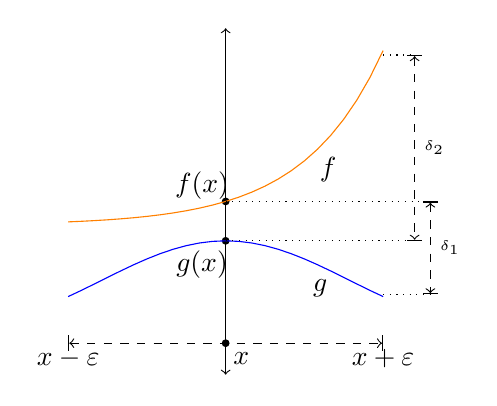
\begin{tikzpicture}[domain=-2:2]
%\draw[very thin,color=gray] (-0.1,-1.1) grid (3.9,3.9);
\draw[dashed, |<->|]   (-2,0) -- (2,0);
\draw[<->] (0,-0.4) -- (0,4); % node[above] {$f(x)$};

    \node at (0,0)[circle,fill,inner sep=1pt]{};
%    \node at (-2,0)[circle,fill,inner sep=1pt]{};
%    \node at (2,0)[circle,fill,inner sep=1pt]{};
\node(z) at (0.2,-0.2) {$x$};
\node(-e) at (-2,-0.2) {$x-\varepsilon$};
\node(e) at (2,-0.2) {$x+\varepsilon$};


\node(f) at (0,0.8+0.5)[circle,fill,inner sep=1pt]{};
\node(f) at (0,1.5+0.3)[circle,fill,inner sep=1pt]{};

\node(f) at (-0.3,2) {$f(x)$};

\node(f) at (-0.3,1) {$g(x)$};


\node(ff) at (1.3,2.2) {{$f$}};
\node(gg) at (1.2,0.7) {{$g$}};

%\draw[color=red] plot (\x,\x) node[right] {$f(x) =x$};
% \x r means to convert ?\x? from degrees to _r_adians:
\draw[color=blue] plot (\x,{0.8+ 0.5*(cos(\x r))}) ;
\draw[color=orange] plot (\x,{1.5+0.3*exp(\x)}) ;

\draw[dotted] (0,1.8) -- (2.6,1.8);
\draw[dotted] (2,0.62) -- (2.6,0.62);
\draw[dotted] (0,1.3) -- (2.4,1.3);
\draw[dotted] (2,3.66) -- (2.4,3.66);

%
%\draw[dotted] (0,1.8) -- (2, 0.62);
%\draw[dotted] (0,1.3) -- (2, 3.66);

\draw[dashed,|<->| ] (2.4,3.66) -- node[right] {\tiny$\delta_{2}$} (2.4,1.3);
\draw[dashed,|<->| ] (2.6,1.8) -- node[right] {\tiny$\delta_{1}$} (2.6,0.62);

\end{tikzpicture}
}
\caption{\small In differential logical relations the distance between two functions $f,g:\R\to \R$, computed at $(x,\varepsilon)$ is the maximum between 
$\delta_{1}=\max\{d(f(x),g(y));~ y\in [x-\varepsilon, x+\varepsilon]\}$ and 
$\delta_{2}=\max\{d(g(x), f(y));~ y\in [x-\varepsilon, x+\varepsilon]\}$.}
% and 
%
%
%minimum $\delta$ such that for all $y\in [x-\varepsilon, x+\varepsilon]$, both $g(y)\in [f(x)-\delta, f(x)+\delta]$ and $f(y)\in[g(x)-\delta, g(x)+\delta]$ hold. $\delta$ is thus $\max\{\delta_{1},\delta_{2}\}$ in the image above.}
\label{fig:graph1}
\end{subfigure} \ \ \ \ 
\begin{subfigure}{0.45\textwidth}
\parbox[h][4.6cm][c]{\textwidth}{
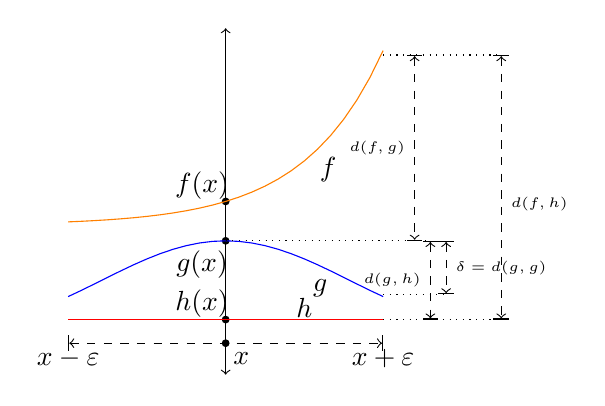
\begin{tikzpicture}[domain=-2:2]
%\draw[very thin,color=gray] (-0.1,-1.1) grid (3.9,3.9);
\draw[dashed, |<->|]   (-2,0) -- (2,0);
\draw[<->] (0,-0.4) -- (0,4); % node[above] {$f(x)$};

    \node at (0,0)[circle,fill,inner sep=1pt]{};
%    \node at (-2,0)[circle,fill,inner sep=1pt]{};
%    \node at (2,0)[circle,fill,inner sep=1pt]{};
\node(z) at (0.2,-0.2) {$x$};
\node(-e) at (-2,-0.2) {$x-\varepsilon$};
\node(e) at (2,-0.2) {$x+\varepsilon$};


\node(f) at (0,0.8+0.5)[circle,fill,inner sep=1pt]{};
\node(f) at (0,1.5+0.3)[circle,fill,inner sep=1pt]{};
\node(f) at (0,0.3)[circle,fill,inner sep=1pt]{};

\node(f) at (-0.3,2) {$f(x)$};

\node(f) at (-0.3,1) {$g(x)$};

\node(f) at (-0.3,0.5) {$h(x)$};

\node(ff) at (1.3,2.2) {{$f$}};
\node(gg) at (1.2,0.7) {{$g$}};
\node(gg) at (1,0.45) {{$h$}};

%\draw[color=red] plot (\x,\x) node[right] {$f(x) =x$};
% \x r means to convert ?\x? from degrees to _r_adians:
\draw[color=blue] plot (\x,{0.8+ 0.5*(cos(\x r))}) ;
\draw[color=orange] plot (\x,{1.5+0.3*exp(\x)}) ;
\draw[color=red] plot (\x,{0.3}) ;



\draw[dotted] (0,1.3) -- (2.6,1.3);
\draw[dotted] (2,0.3) -- (3.5,0.3);
\draw[dotted] (0,1.3) -- (2.4,1.3);
\draw[dotted] (2,3.66) -- (3.5,3.66);
\draw[dotted] (2,0.62) -- (2.8,0.62);

%
%\draw[dotted] (0,1.8) -- (2, 0.62);
%\draw[dotted] (0,1.3) -- (2, 3.66);

\draw[dashed,|<->| ] (2.4,3.66) -- node[left] {\tiny$d(f,g)$} (2.4,1.3);
\draw[dashed,|<->| ] (2.6,1.3) -- node[left] {\tiny$d(g,h)$} (2.6,0.3);

\draw[dashed,|<->| ] (2.8,1.3) -- node[right] {\tiny$\delta=d(g,g)$} (2.8,0.62);

%\draw[dashed,|<->| ] (3.5,2.96) -- node[above right] {\tiny$\begin{matrix}d(f,g)+d(g,h)\\ -d(g,g)\end{matrix}$} (3.5,0.3);

\draw[dashed,|<->| ] (3.5,3.66) -- node[below right] {\tiny$d(f,h)$} (3.5,0.3);

\end{tikzpicture}
}
%
\caption{\small The distance arising from differential logical relations is not a partial metric: the example above shows that $d(f,h)> d(f,g)+d(g,h)- d(g,g)$ (with all distances computed in $(x,\varepsilon)$).}% and 
%
%
%minimum $\delta$ such that for all $y\in [x-\varepsilon, x+\varepsilon]$, both $g(y)\in [f(x)-\delta, f(x)+\delta]$ and $f(y)\in[g(x)-\delta, g(x)+\delta]$ hold. $\delta$ is thus $\max\{\delta_{1},\delta_{2}\}$ in the image above.}
\label{fig:graph2}
\end{subfigure}
\end{figure}

\subparagraph*{Related work}


A primary source of inspiration for our approach was the recent work of Dal Lago, Gavazzo and Yoshimizu on  \emph{differential logical relations} \cite{dallago:differential-stlc}. This is a semantics for higher-order languages in which a type is interpreted as a set $X$ endowed with a kind of metric structure expressed by a relation $\rho \subseteq X\times \mathbb Q\times X$, where $\mathbb Q$ is an arbitrary quantale. To our knowledge, this is the first place were the idea of varying the quantales in which distances are measured is introduced as a key ingredient to obtain a cartesian closed category.

While the relation $\rho$ of a GMS induces a distance function $d_{\rho}(x,y)=\sup\{\epsilon\mid \rho(x,\epsilon,y)\}$, this function is not a partial metric. We can show this fact with a simple example: in this model the distance between two programs 
 $f,g:\mathsf{Real}\to \mathsf{Real}$ is taken in the quantale of functions from $\R\times \R_{+}^{\infty}$ to $\R_{+}^{\infty}$: intuitively, 
  $d(f,g)$ associates a closed interval $[x-\epsilon,x+\epsilon]$ (corresponding to the pair $(x,\varepsilon)$) with the smallest distance $\delta$ such that $[ f(x)-\delta, f(x)+\delta]$ and $[g(x)-\delta,g(x)+\delta]$ both contain the images of $[x-\varepsilon, x+\varepsilon]$ through
 $g$ and $f$ respectively (see Fig. \ref{fig:graph1}). Then, as shown in Fig. \ref{fig:graph2}, by letting $\delta=d(g,g)(x,\varepsilon)$, we have that $d(g,g)$ sends the interval $I=[x-\varepsilon, x+\varepsilon]$ onto the interval $[g(x)-\delta, g(x)+\delta]$, which has diameter $2\delta$, while the image of $I$ has diameter $\delta$, making the triangular law of partial metrics fail. 



A more syntactic approach to approximate program transformations is the one in 
\cite{chaudhuri}, which introduces a System F-based type system with a type of real numbers and an explicit distinction between exact and approximate programs.
%, and provides typing rules to formalize contextual reasoning about program differences. As in the case of differential logical relations, program differences are taken as functions relating errors in input and errors in output, but the viewpoint of program metric is not considered.
Like the case of loop perforation discussed in Section 4, most examples of contextual reasoning from \cite{chaudhuri} can be  reformulated in our framework. 




The literature on program pseudo-metrics is vast. A major distinction can be made between those approaches in which metrics account for \emph{extensional} aspects of programs (like ours), 
 and approaches in which metrics are used to characterize \emph{intensional} aspects.
To the first family belong all metric models developed for reasoning about differential privacy \cite{},  
probabilistic computation \cite{} and co-inductive models \cite{}.
%In particular, several approaches like \cite{} emphasize the importance to formalize contextual reasoning, wich can be assured in frameworks like \cite{} by the restriction to Lipschitz-continuous or non-expansive functions. 
To the second class belong approaches like \cite{} which recovers the Scott model of PCF through a ultrametric semantics, as well as most of previous models based on partial metric spaces, which rely on a correspondence between continuous Scott domains and the $T_{1}$ topology of partial metrics.
%
%. 
%The central motivation such approaches is the observation that a partial metric $d$ on a set $X$ induces an order relation given by $x\preceq_{d}y$ iff $d(x,y)\leq d(x,x)$, turning $X$ into a continuous Scott domain and, conversely, any continuous Scott domain with a countable basis is induced by a partial metric in this way.
%This allows to reformulate several classical results on denotational semantics using the $T_{1}$ topology of partial metric spaces.
%


More recently, \cite{Stubbe} introduced an elegant categorical approach to GPMS in the framework of \emph{quantaloid-enriched categories}, as well as a 
characterization of exponentiable GPMS, showing in particular that no such category can be both cartesian closed categories and contain the standard metric on $\mathbb R$. This result seems to add further evidence of the necessity of considering metrics over varying quantales in order to model higher-order languages. 
%
%While in all these results distances are computed over a \emph{fixed} quantale, the generalization of this categorical approach to varying quantales seems to be a yet unexplored research direction.






\subparagraph*{Future work}


%
%
%In this paper we constructed a (non-extensional) model of the simply typed $\lambda$-calculus based on generalized partial metric spaces. Our model provides a 
% differential semantics of higher-order programs, that is, a semantic description of \emph{differences} between
% higher-order programs. 
% The main novelty is that we take as morphisms between metric spaces approximate functions, \emph{i.e.} monotone functions over intervals, rather than continuous functions of some kind. While approximate functions represent sets of similar programs, usual, exact, programs can be embedded in the model through a differentiation operator. 
% This approach allows us to overcome the well-known obstacle that usual categories of metric spaces and continuous functions are not cartesian closed, and therefore cannot be models of $\STLC$.
%% 
% Instead, we obtain 
%based on generalized partial metric spaces and
%
%Moreover, our model refines previous notions of program distances based on differential logical relations.
%
%
%the use of partial metric spaces, a well-investigated metric structure to which most fundamental properties and results on standard metric spaces scale well, 
%
%
%
%
%. More importantly, we take, as morphisms between them, approximate functions, that is, function over closed intervals, rather than (Lipschitz-) continuous or non-expansive functions over points, as in usual categories of metric spaces.

The approach we presented lends itself to further extensions and generalizations.
First, we would like to investigate the interpretation of more type constructions than those of $\STLC$ (e.g. sum types, recursive types, effects). Moreover, we would like to explore the possibility of exploiting the structure of the category $\dsp(\mathbb C)$ to construct new and more refined notions of approximations.
For example (we work in $\dsp(\set))$ for simplicity), 
starting from the ``standard'' set of approximate values $\mathcal I$ on $\mathbb{R}^{X\times X}$ (with elements of $\mathcal I$ being  families of compact intervals $U_{x,x'}\subseteq \mathbb R$ indexed by values in $X\times X$), one can define a new family  $\Delta^{*}\mathcal I$  of approximate values for  $\mathbb R^{X}$ by ``pulling back'' the exact map 
$\Delta:
\mathbb R^{X} \to \mathbb R^{X\times X}$ defined by $\Delta f(x,x')=f(x')-f(x)$. 
The new approximate values corresponds then to sets of functions $f\in \mathbb R^{X}$ with a controlled variation, that is, such that $f(x')-f(x)$ is bounded by some family of intervals $U_{x,x'} \in \mathcal I$.





%
%First, in this paper we restricted our attention to $\STLC$, which is not a universal language. 
%The accommodation of full recursion in metric models is usually obtained by an application of the Banach fixed point theorem \cite{VANBREUGEL20011}. As this theorem scales well to partial metric spaces \cite{Samet:2013aa}, a natural question is whether our model, or some variant of it, can be used to provide a metric account of universal computation over the real numbers.
%


Another interesting research direction concerns probabilistic extensions of $\STLC$. 
Probabilistic metrics \cite{1029849,KOZEN1981328, 10.1109/LICS.2015.64, 10.1007/978-3-662-54434-1_13} have been the object of much research in recent years, due to the relevance of metric reasoning in some areas of computer science in which probabilistic computation plays a key role (e.g. in cryptography \cite{GOLDWASSER1984270} and machine learning \cite{krause08robust}).
A convenient starting point seems to be the recent generalization of {probabilistic (generalized) metric spaces} to the partial metric case \cite{HE201999}.




